%%%%%%%%%%%%%%%%%%%%%%%%%%%%%%%%%%%%%%%%%
% Template
% LaTeX Template
% Version 1.0 (December 8 2014)
%
% This template has been downloaded from:
% http://www.LaTeXTemplates.com
%
% Original author:
% Brandon Fryslie
% With extensive modifications by:
% Vel (vel@latextemplates.com)
%
% License:
% CC BY-NC-SA 3.0 (http://creativecommons.org/licenses/by-nc-sa/3.0/)
%
% Authors:
% Sabbir Ahmed
% 
%%%%%%%%%%%%%%%%%%%%%%%%%%%%%%%%%%%%%%%%%

\documentclass[paper=usletter, fontsize=12pt]{article}
%%%%%%%%%%%%%%%%%%%%%%%%%%%%%%%%%%%%%%%%%
% Contract Structural Definitions File Version 1.0 (December 8 2014)
%
% Created by: Vel (vel@latextemplates.com)
% 
% This file has been downloaded from: http://www.LaTeXTemplates.com
%
% License: CC BY-NC-SA 3.0 (http://creativecommons.org/licenses/by-nc-sa/3.0/)
%
%%%%%%%%%%%%%%%%%%%%%%%%%%%%%%%%%%%%%%%%%

\usepackage{geometry} % Required to modify the page layout
\usepackage{multicol}
\usepackage{amsmath}
\usepackage{amssymb}

\usepackage[pdftex]{graphicx}
\usepackage{wrapfig}
\usepackage[font=scriptsize, labelfont=bf]{caption}
\usepackage[utf8]{inputenc} % Required for including letters with accents
\usepackage[T1]{fontenc} % Use 8-bit encoding that has 256 glyphs

\usepackage{avant} % Use the Avantgarde font for headings
\usepackage{courier}
\usepackage{xparse}
\usepackage{xcolor}
\usepackage{listings}  % for code verbatim and console outputs

\setlength{\textwidth}{16cm} % Width of the text on the page
\setlength{\textheight}{23cm} % Height of the text on the page
\setlength{\oddsidemargin}{0cm} % Width of the margin - negative to move text left, positive to move it right
\setlength{\topmargin}{-1.25cm} % Reduce the top margin

\setlength{\parindent}{0mm} % Don't indent paragraphs
\setlength{\parskip}{2.5mm} % Whitespace between paragraphs
\renewcommand{\baselinestretch}{1.5}

\definecolor{green}{rgb}{0.18, 0.55, 0.34}

\graphicspath{ {figures/} }
\captionsetup[table]{skip=10pt}

\lstset{language=C, keywordstyle={\bfseries \color{black}}}

% defines algorithm counter for chapter-level
\newcounter{nalg}[section]

%defines appearance of the algorithm counter
\renewcommand{\thenalg}{\thesection .\arabic{nalg}}

% defines a new caption label as Algorithm x.y
\DeclareCaptionLabelFormat{algocaption}{Algorithm \thenalg}

% defines the algorithm listing environment
\lstnewenvironment{pseudocode}[1][] {
    \refstepcounter{nalg}  % increments algorithm number
    \captionsetup{font=normalsize, labelformat=algocaption, labelsep=colon}
    \lstset{
        breaklines=true,
        mathescape=true,
        numbers=left,
        numberstyle=\scriptsize,
        basicstyle=\footnotesize\ttfamily,
        keywordstyle=\color{black}\bfseries,
        keywords={input, output, return, parallel, function, for, to, in, if,
        else, foreach, while, and, or, new, print},
        xleftmargin=.04\textwidth,
        #1
    }
}{}

\renewcommand{\familydefault}{\sfdefault}  % default font for entire document
 % specifies the document layout and style

\begin{document}

    \documentinfo{\textbf{Homework 3: Light the Candles}}{\textbf{Date:} \today}{Sabbir Ahmed}
    \vspace{-0.1in}

    \section{Background}
    For this assignment, a game was created to be played on the development board. The goal of the game is for the player to light all the candles, represented by the 8 LEDs on the board just above the switches, while they are being pseudo-randomly turned off.
    
    The game starts off with the player pressing the RESET button (a.k.a. BTN\_SOUTH) just below the rotatory knob.

    The player is placed initially at a position 0.

    The player may light the candles by jumping on them. This is done using the BTN\_NORTH button on the board just above the rotary knob. A player may jump at the current position by setting the switches to zero and pressing BTN\_NORTH. Any desired horizontal movement in the jump to another position is provide by the four switches which indicate a value from 7 to -8, in binary two's compliment.

    Once a candle is lit, the player may jump again jump on the same location (using 0) or to another location using the delta provide by the switches.

    However, the candles that were lit will continually go out at random and must be relit. To be specific, a candle may at random go out at the same time the player jumps. Secondly, note that there is no direct indicator to where the player is; so it is up to the player to keep track.

    \section{Implementation}
    Three discrete modules were used to implement the game: \inlsnip{igniter}, \inlsnip{extinguisher} and \inlsnip{candle_controller}. These submodules were connected and debounced using a top level module that may be visualized with the the block diagram and the schematic diagram in Figures \ref{fig:block} and \ref{fig:schematic}.

    \begin{figure}[ht]
        \begin{center}
            \includegraphics[width=1\textwidth]{block.png}
            \caption{Schematic of the Implementation of the Game} \label{fig:block}
        \end{center}
    \end{figure}

    \begin{figure}[ht]
        \begin{center}
            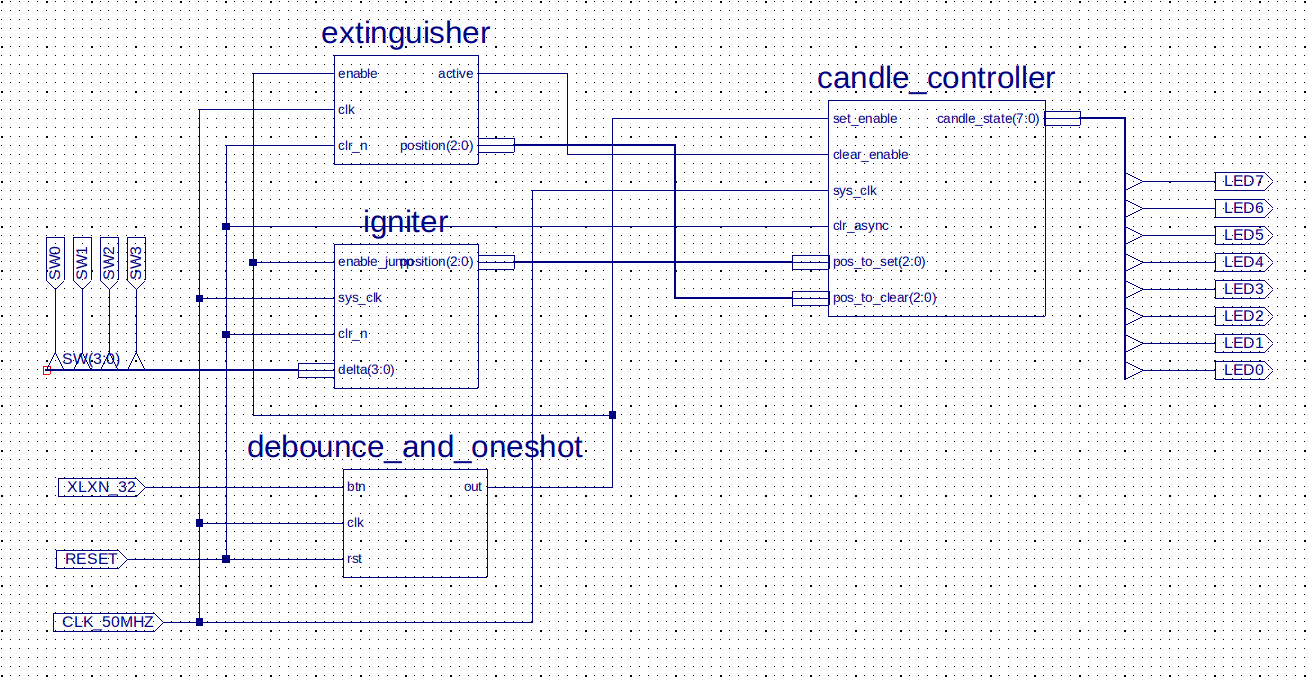
\includegraphics[width=1\textwidth]{schematic.png}
            \caption{Schematic of the Implementation of the Game} \label{fig:schematic}
        \end{center}
    \end{figure}

\end{document}
